% Options for packages loaded elsewhere
\PassOptionsToPackage{unicode}{hyperref}
\PassOptionsToPackage{hyphens}{url}
%
\documentclass[
]{article}
\usepackage{amsmath,amssymb}
\usepackage{iftex}
\ifPDFTeX
  \usepackage[T1]{fontenc}
  \usepackage[utf8]{inputenc}
  \usepackage{textcomp} % provide euro and other symbols
\else % if luatex or xetex
  \usepackage{unicode-math} % this also loads fontspec
  \defaultfontfeatures{Scale=MatchLowercase}
  \defaultfontfeatures[\rmfamily]{Ligatures=TeX,Scale=1}
\fi
\usepackage{lmodern}
\ifPDFTeX\else
  % xetex/luatex font selection
\fi
% Use upquote if available, for straight quotes in verbatim environments
\IfFileExists{upquote.sty}{\usepackage{upquote}}{}
\IfFileExists{microtype.sty}{% use microtype if available
  \usepackage[]{microtype}
  \UseMicrotypeSet[protrusion]{basicmath} % disable protrusion for tt fonts
}{}
\makeatletter
\@ifundefined{KOMAClassName}{% if non-KOMA class
  \IfFileExists{parskip.sty}{%
    \usepackage{parskip}
  }{% else
    \setlength{\parindent}{0pt}
    \setlength{\parskip}{6pt plus 2pt minus 1pt}}
}{% if KOMA class
  \KOMAoptions{parskip=half}}
\makeatother
\usepackage{xcolor}
\usepackage[margin=1in]{geometry}
\usepackage{color}
\usepackage{fancyvrb}
\newcommand{\VerbBar}{|}
\newcommand{\VERB}{\Verb[commandchars=\\\{\}]}
\DefineVerbatimEnvironment{Highlighting}{Verbatim}{commandchars=\\\{\}}
% Add ',fontsize=\small' for more characters per line
\usepackage{framed}
\definecolor{shadecolor}{RGB}{248,248,248}
\newenvironment{Shaded}{\begin{snugshade}}{\end{snugshade}}
\newcommand{\AlertTok}[1]{\textcolor[rgb]{0.94,0.16,0.16}{#1}}
\newcommand{\AnnotationTok}[1]{\textcolor[rgb]{0.56,0.35,0.01}{\textbf{\textit{#1}}}}
\newcommand{\AttributeTok}[1]{\textcolor[rgb]{0.13,0.29,0.53}{#1}}
\newcommand{\BaseNTok}[1]{\textcolor[rgb]{0.00,0.00,0.81}{#1}}
\newcommand{\BuiltInTok}[1]{#1}
\newcommand{\CharTok}[1]{\textcolor[rgb]{0.31,0.60,0.02}{#1}}
\newcommand{\CommentTok}[1]{\textcolor[rgb]{0.56,0.35,0.01}{\textit{#1}}}
\newcommand{\CommentVarTok}[1]{\textcolor[rgb]{0.56,0.35,0.01}{\textbf{\textit{#1}}}}
\newcommand{\ConstantTok}[1]{\textcolor[rgb]{0.56,0.35,0.01}{#1}}
\newcommand{\ControlFlowTok}[1]{\textcolor[rgb]{0.13,0.29,0.53}{\textbf{#1}}}
\newcommand{\DataTypeTok}[1]{\textcolor[rgb]{0.13,0.29,0.53}{#1}}
\newcommand{\DecValTok}[1]{\textcolor[rgb]{0.00,0.00,0.81}{#1}}
\newcommand{\DocumentationTok}[1]{\textcolor[rgb]{0.56,0.35,0.01}{\textbf{\textit{#1}}}}
\newcommand{\ErrorTok}[1]{\textcolor[rgb]{0.64,0.00,0.00}{\textbf{#1}}}
\newcommand{\ExtensionTok}[1]{#1}
\newcommand{\FloatTok}[1]{\textcolor[rgb]{0.00,0.00,0.81}{#1}}
\newcommand{\FunctionTok}[1]{\textcolor[rgb]{0.13,0.29,0.53}{\textbf{#1}}}
\newcommand{\ImportTok}[1]{#1}
\newcommand{\InformationTok}[1]{\textcolor[rgb]{0.56,0.35,0.01}{\textbf{\textit{#1}}}}
\newcommand{\KeywordTok}[1]{\textcolor[rgb]{0.13,0.29,0.53}{\textbf{#1}}}
\newcommand{\NormalTok}[1]{#1}
\newcommand{\OperatorTok}[1]{\textcolor[rgb]{0.81,0.36,0.00}{\textbf{#1}}}
\newcommand{\OtherTok}[1]{\textcolor[rgb]{0.56,0.35,0.01}{#1}}
\newcommand{\PreprocessorTok}[1]{\textcolor[rgb]{0.56,0.35,0.01}{\textit{#1}}}
\newcommand{\RegionMarkerTok}[1]{#1}
\newcommand{\SpecialCharTok}[1]{\textcolor[rgb]{0.81,0.36,0.00}{\textbf{#1}}}
\newcommand{\SpecialStringTok}[1]{\textcolor[rgb]{0.31,0.60,0.02}{#1}}
\newcommand{\StringTok}[1]{\textcolor[rgb]{0.31,0.60,0.02}{#1}}
\newcommand{\VariableTok}[1]{\textcolor[rgb]{0.00,0.00,0.00}{#1}}
\newcommand{\VerbatimStringTok}[1]{\textcolor[rgb]{0.31,0.60,0.02}{#1}}
\newcommand{\WarningTok}[1]{\textcolor[rgb]{0.56,0.35,0.01}{\textbf{\textit{#1}}}}
\usepackage{longtable,booktabs,array}
\usepackage{calc} % for calculating minipage widths
% Correct order of tables after \paragraph or \subparagraph
\usepackage{etoolbox}
\makeatletter
\patchcmd\longtable{\par}{\if@noskipsec\mbox{}\fi\par}{}{}
\makeatother
% Allow footnotes in longtable head/foot
\IfFileExists{footnotehyper.sty}{\usepackage{footnotehyper}}{\usepackage{footnote}}
\makesavenoteenv{longtable}
\usepackage{graphicx}
\makeatletter
\def\maxwidth{\ifdim\Gin@nat@width>\linewidth\linewidth\else\Gin@nat@width\fi}
\def\maxheight{\ifdim\Gin@nat@height>\textheight\textheight\else\Gin@nat@height\fi}
\makeatother
% Scale images if necessary, so that they will not overflow the page
% margins by default, and it is still possible to overwrite the defaults
% using explicit options in \includegraphics[width, height, ...]{}
\setkeys{Gin}{width=\maxwidth,height=\maxheight,keepaspectratio}
% Set default figure placement to htbp
\makeatletter
\def\fps@figure{htbp}
\makeatother
\setlength{\emergencystretch}{3em} % prevent overfull lines
\providecommand{\tightlist}{%
  \setlength{\itemsep}{0pt}\setlength{\parskip}{0pt}}
\setcounter{secnumdepth}{-\maxdimen} % remove section numbering
\usepackage{multirow}
\usepackage{multicol}
\usepackage{colortbl}
\usepackage{hhline}
\newlength\Oldarrayrulewidth
\newlength\Oldtabcolsep
\usepackage{longtable}
\usepackage{array}
\usepackage{hyperref}
\usepackage{float}
\usepackage{wrapfig}
\usepackage{booktabs}
\usepackage{caption}
\ifLuaTeX
  \usepackage{selnolig}  % disable illegal ligatures
\fi
\IfFileExists{bookmark.sty}{\usepackage{bookmark}}{\usepackage{hyperref}}
\IfFileExists{xurl.sty}{\usepackage{xurl}}{} % add URL line breaks if available
\urlstyle{same}
\hypersetup{
  pdftitle={Introduction to R-Markdown},
  pdfauthor={Arjun},
  hidelinks,
  pdfcreator={LaTeX via pandoc}}

\title{Introduction to R-Markdown}
\author{Arjun}
\date{2024-01-19}

\begin{document}
\maketitle

Include a first-level header, second-level header, and third-level
header in your R Markdown document naming them Section 1, Subsection 1,
and Subsubsection 1, respectively.

\hypertarget{section-1}{%
\section{Section 1}\label{section-1}}

This is first level header

\hypertarget{subsection-1-section-2}{%
\subsection{Subsection 1: Section 2}\label{subsection-1-section-2}}

This is a second level header

\hypertarget{subsubsection-1-section-3}{%
\subsubsection{Subsubsection 1: Section
3}\label{subsubsection-1-section-3}}

This is a third level header

Include a hyperlink in the R Markdown document linking to the Google
homepage.

\url{http://www.google.com}

or

\href{http://www.google.com}{Google Home}

\begin{figure}
\centering
\includegraphics{https://media.istockphoto.com/id/1317323736/photo/a-view-up-into-the-trees-direction-sky.jpg?s=1024x1024\&w=is\&k=20\&c=9Qfj9S124ojed7s4OWu3a3vbbMC76QYkqczg4L4M-Sc=}
\caption{Here is an image}
\end{figure}

\hypertarget{different-formats-of-text}{%
\subsubsection{Different formats of
text}\label{different-formats-of-text}}

\textbf{Bold} text.

\emph{Italicized} text.

\texttt{code} style text.

subscript\textsubscript{PM}

superscript\textsuperscript{AM}

\hypertarget{add-a-new-code-chunk-at-the-bottom-of-the-r-markdown-document-naming-the-chunk-uptownchunk.-in-the-chunk-use-the-include_graphics-function-from-the-knitr-package-to-include-the-image-at-the-following-url-httpsgithub.comdilerniasta418-518blobmainuptownfunk.pngrawtrue}{%
\paragraph{\texorpdfstring{Add a new code chunk at the bottom of the R
Markdown document, naming the chunk uptownChunk. In the chunk, use the
include\_graphics() function from the knitr package to include the image
at the following URL:
\url{https://github.com/dilernia/STA418-518/blob/main/uptownFunk.png?raw=true}}{Add a new code chunk at the bottom of the R Markdown document, naming the chunk uptownChunk. In the chunk, use the include\_graphics() function from the knitr package to include the image at the following URL: https://github.com/dilernia/STA418-518/blob/main/uptownFunk.png?raw=true}}\label{add-a-new-code-chunk-at-the-bottom-of-the-r-markdown-document-naming-the-chunk-uptownchunk.-in-the-chunk-use-the-include_graphics-function-from-the-knitr-package-to-include-the-image-at-the-following-url-httpsgithub.comdilerniasta418-518blobmainuptownfunk.pngrawtrue}}

\includegraphics{https://github.com/dilernia/STA418-518/blob/main/uptownFunk.png?raw=true}

Let's make a scatterplot

\begin{Shaded}
\begin{Highlighting}[]
\FunctionTok{library}\NormalTok{(tidyverse)}
\end{Highlighting}
\end{Shaded}

\begin{verbatim}
## Warning: package 'tidyverse' was built under R version 4.3.2
\end{verbatim}

\begin{verbatim}
## Warning: package 'ggplot2' was built under R version 4.3.2
\end{verbatim}

\begin{verbatim}
## Warning: package 'dplyr' was built under R version 4.3.2
\end{verbatim}

\begin{verbatim}
## -- Attaching core tidyverse packages ------------------------ tidyverse 2.0.0 --
## v dplyr     1.1.3     v readr     2.1.4
## v forcats   1.0.0     v stringr   1.5.1
## v ggplot2   3.4.4     v tibble    3.2.1
## v lubridate 1.9.3     v tidyr     1.3.0
## v purrr     1.0.2     
## -- Conflicts ------------------------------------------ tidyverse_conflicts() --
## x dplyr::filter() masks stats::filter()
## x dplyr::lag()    masks stats::lag()
## i Use the conflicted package (<http://conflicted.r-lib.org/>) to force all conflicts to become errors
\end{verbatim}

\begin{Shaded}
\begin{Highlighting}[]
\CommentTok{\# Load storms data set}
\FunctionTok{data}\NormalTok{(storms)}

\NormalTok{storms }\SpecialCharTok{|\textgreater{}} \FunctionTok{ggplot}\NormalTok{(}\FunctionTok{aes}\NormalTok{(}\AttributeTok{x =}\NormalTok{ pressure, }\AttributeTok{y =}\NormalTok{ wind)) }\SpecialCharTok{+} 
  \FunctionTok{geom\_point}\NormalTok{()}
\end{Highlighting}
\end{Shaded}

\begin{center}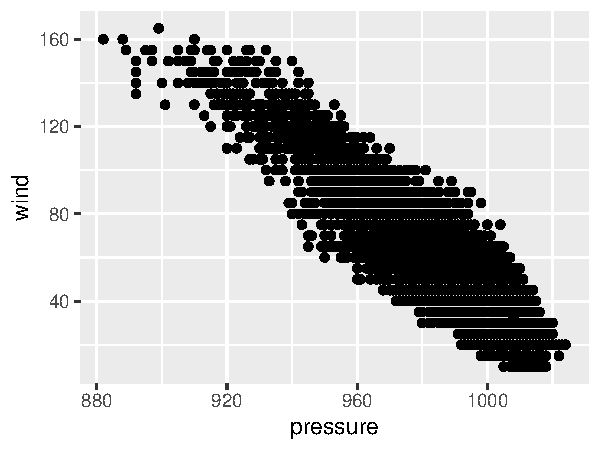
\includegraphics{Introduction-to-RMarkdown_files/figure-latex/unnamed-chunk-1-1} \end{center}

\hypertarget{inline-code}{%
\paragraph{Inline code}\label{inline-code}}

The 95\% confidence interval for the mean is (-0.548, 4.548).

This is an example for inline code.

\hypertarget{tables}{%
\subsection{Tables}\label{tables}}

\begin{Shaded}
\begin{Highlighting}[]
\CommentTok{\# Seven largest sustained wind speeds recorded}
\NormalTok{storms\_summary }\OtherTok{\textless{}{-}}\NormalTok{ storms }\SpecialCharTok{|\textgreater{}} 
  \FunctionTok{group\_by}\NormalTok{(name, year) }\SpecialCharTok{|\textgreater{}} 
  \FunctionTok{summarize}\NormalTok{(}\AttributeTok{max\_wind\_knots =} \FunctionTok{max}\NormalTok{(wind)) }\SpecialCharTok{|\textgreater{}} 
  \FunctionTok{ungroup}\NormalTok{() }\SpecialCharTok{|\textgreater{}} 
  \FunctionTok{slice\_max}\NormalTok{(max\_wind\_knots, }\AttributeTok{n =} \DecValTok{4}\NormalTok{)}
\end{Highlighting}
\end{Shaded}

\begin{verbatim}
## `summarise()` has grouped output by 'name'. You can override using the
## `.groups` argument.
\end{verbatim}

\begin{Shaded}
\begin{Highlighting}[]
\FunctionTok{library}\NormalTok{(knitr)}
\end{Highlighting}
\end{Shaded}

\begin{verbatim}
## Warning: package 'knitr' was built under R version 4.3.2
\end{verbatim}

\begin{Shaded}
\begin{Highlighting}[]
\NormalTok{storms\_summary }\SpecialCharTok{|\textgreater{}} 
  \FunctionTok{kable}\NormalTok{(}\AttributeTok{caption =} \StringTok{"Table 1. Storm summary statistics with kable()"}\NormalTok{)}
\end{Highlighting}
\end{Shaded}

\begin{longtable}[]{@{}lrr@{}}
\caption{Table 1. Storm summary statistics with kable()}\tabularnewline
\toprule\noalign{}
name & year & max\_wind\_knots \\
\midrule\noalign{}
\endfirsthead
\toprule\noalign{}
name & year & max\_wind\_knots \\
\midrule\noalign{}
\endhead
\bottomrule\noalign{}
\endlastfoot
Allen & 1980 & 165 \\
Dorian & 2019 & 160 \\
Gilbert & 1988 & 160 \\
Wilma & 2005 & 160 \\
\end{longtable}

\begin{Shaded}
\begin{Highlighting}[]
\FunctionTok{library}\NormalTok{(flextable)}
\end{Highlighting}
\end{Shaded}

\begin{verbatim}
## Warning: package 'flextable' was built under R version 4.3.2
\end{verbatim}

\begin{verbatim}
## 
## Attaching package: 'flextable'
\end{verbatim}

\begin{verbatim}
## The following object is masked from 'package:purrr':
## 
##     compose
\end{verbatim}

\begin{Shaded}
\begin{Highlighting}[]
\NormalTok{storms\_summary }\SpecialCharTok{|\textgreater{}} 
  \FunctionTok{flextable}\NormalTok{() }\SpecialCharTok{|\textgreater{}} 
  \FunctionTok{set\_caption}\NormalTok{(}\AttributeTok{caption =} \StringTok{"Table 1. Storm summary statistics with flextable()"}\NormalTok{) }\SpecialCharTok{|\textgreater{}} 
  \FunctionTok{colformat\_double}\NormalTok{(}\AttributeTok{big.mark =} \StringTok{""}\NormalTok{, }\AttributeTok{digits =} \DecValTok{0}\NormalTok{) }\SpecialCharTok{|\textgreater{}} 
  \FunctionTok{autofit}\NormalTok{()}
\end{Highlighting}
\end{Shaded}

\begin{verbatim}
## Warning: fonts used in `flextable` are ignored because the `pdflatex` engine is
## used and not `xelatex` or `lualatex`. You can avoid this warning by using the
## `set_flextable_defaults(fonts_ignore=TRUE)` command or use a compatible engine
## by defining `latex_engine: xelatex` in the YAML header of the R Markdown
## document.
\end{verbatim}

\global\setlength{\Oldarrayrulewidth}{\arrayrulewidth}

\global\setlength{\Oldtabcolsep}{\tabcolsep}

\setlength{\tabcolsep}{0pt}

\renewcommand*{\arraystretch}{1.5}



\providecommand{\ascline}[3]{\noalign{\global\arrayrulewidth #1}\arrayrulecolor[HTML]{#2}\cline{#3}}

\begin{longtable}[c]{|p{0.74in}|p{0.63in}|p{1.42in}}

\caption{Table\ 1.\ Storm\ summary\ statistics\ with\ flextable()}\\

\ascline{1.5pt}{666666}{1-3}

\multicolumn{1}{>{\raggedright}m{\dimexpr 0.74in+0\tabcolsep}}{\textcolor[HTML]{000000}{\fontsize{11}{11}\selectfont{name}}} & \multicolumn{1}{>{\raggedleft}m{\dimexpr 0.63in+0\tabcolsep}}{\textcolor[HTML]{000000}{\fontsize{11}{11}\selectfont{year}}} & \multicolumn{1}{>{\raggedleft}m{\dimexpr 1.42in+0\tabcolsep}}{\textcolor[HTML]{000000}{\fontsize{11}{11}\selectfont{max\_wind\_knots}}} \\

\ascline{1.5pt}{666666}{1-3}\endfirsthead \caption[]{Table\ 1.\ Storm\ summary\ statistics\ with\ flextable()}\\

\ascline{1.5pt}{666666}{1-3}

\multicolumn{1}{>{\raggedright}m{\dimexpr 0.74in+0\tabcolsep}}{\textcolor[HTML]{000000}{\fontsize{11}{11}\selectfont{name}}} & \multicolumn{1}{>{\raggedleft}m{\dimexpr 0.63in+0\tabcolsep}}{\textcolor[HTML]{000000}{\fontsize{11}{11}\selectfont{year}}} & \multicolumn{1}{>{\raggedleft}m{\dimexpr 1.42in+0\tabcolsep}}{\textcolor[HTML]{000000}{\fontsize{11}{11}\selectfont{max\_wind\_knots}}} \\

\ascline{1.5pt}{666666}{1-3}\endhead



\multicolumn{1}{>{\raggedright}m{\dimexpr 0.74in+0\tabcolsep}}{\textcolor[HTML]{000000}{\fontsize{11}{11}\selectfont{Allen}}} & \multicolumn{1}{>{\raggedleft}m{\dimexpr 0.63in+0\tabcolsep}}{\textcolor[HTML]{000000}{\fontsize{11}{11}\selectfont{1980}}} & \multicolumn{1}{>{\raggedleft}m{\dimexpr 1.42in+0\tabcolsep}}{\textcolor[HTML]{000000}{\fontsize{11}{11}\selectfont{165}}} \\





\multicolumn{1}{>{\raggedright}m{\dimexpr 0.74in+0\tabcolsep}}{\textcolor[HTML]{000000}{\fontsize{11}{11}\selectfont{Dorian}}} & \multicolumn{1}{>{\raggedleft}m{\dimexpr 0.63in+0\tabcolsep}}{\textcolor[HTML]{000000}{\fontsize{11}{11}\selectfont{2019}}} & \multicolumn{1}{>{\raggedleft}m{\dimexpr 1.42in+0\tabcolsep}}{\textcolor[HTML]{000000}{\fontsize{11}{11}\selectfont{160}}} \\





\multicolumn{1}{>{\raggedright}m{\dimexpr 0.74in+0\tabcolsep}}{\textcolor[HTML]{000000}{\fontsize{11}{11}\selectfont{Gilbert}}} & \multicolumn{1}{>{\raggedleft}m{\dimexpr 0.63in+0\tabcolsep}}{\textcolor[HTML]{000000}{\fontsize{11}{11}\selectfont{1988}}} & \multicolumn{1}{>{\raggedleft}m{\dimexpr 1.42in+0\tabcolsep}}{\textcolor[HTML]{000000}{\fontsize{11}{11}\selectfont{160}}} \\





\multicolumn{1}{>{\raggedright}m{\dimexpr 0.74in+0\tabcolsep}}{\textcolor[HTML]{000000}{\fontsize{11}{11}\selectfont{Wilma}}} & \multicolumn{1}{>{\raggedleft}m{\dimexpr 0.63in+0\tabcolsep}}{\textcolor[HTML]{000000}{\fontsize{11}{11}\selectfont{2005}}} & \multicolumn{1}{>{\raggedleft}m{\dimexpr 1.42in+0\tabcolsep}}{\textcolor[HTML]{000000}{\fontsize{11}{11}\selectfont{160}}} \\

\ascline{1.5pt}{666666}{1-3}



\end{longtable}



\arrayrulecolor[HTML]{000000}

\global\setlength{\arrayrulewidth}{\Oldarrayrulewidth}

\global\setlength{\tabcolsep}{\Oldtabcolsep}

\renewcommand*{\arraystretch}{1}

\begin{Shaded}
\begin{Highlighting}[]
\FunctionTok{library}\NormalTok{(gt)}
\end{Highlighting}
\end{Shaded}

\begin{verbatim}
## Warning: package 'gt' was built under R version 4.3.2
\end{verbatim}

\begin{Shaded}
\begin{Highlighting}[]
\NormalTok{storms\_summary }\SpecialCharTok{|\textgreater{}} 
  \FunctionTok{gt}\NormalTok{() }\SpecialCharTok{|\textgreater{}} 
  \FunctionTok{tab\_header}\NormalTok{(}\AttributeTok{title =} \StringTok{"Table 1. Storm summary statistics with gt()"}\NormalTok{)}
\end{Highlighting}
\end{Shaded}

\begin{longtable}{lrr}
\caption*{
{\large Table 1. Storm summary statistics with gt()}
} \\ 
\toprule
name & year & max\_wind\_knots \\ 
\midrule\addlinespace[2.5pt]
Allen & 1980 & 165 \\ 
Dorian & 2019 & 160 \\ 
Gilbert & 1988 & 160 \\ 
Wilma & 2005 & 160 \\ 
\bottomrule
\end{longtable}

\end{document}
